\section{系统实现}

针对以上设计,我们实现了 AquaFS 文件系统。
AquaFS 文件系统的实现基于 ZenFS,我们在 ZenFS 的基础上进行了修改和优化,使其支持 RAID 等功能。

在初赛阶段,由于人手不足等问题,我们优先实现 AquaFS 文件系统的以下几个部分:

\begin{enumerate}
  \item AquaFS 文件系统的 RAID 实现
  \item AquaFS 的 IO 加速实现
  \item AquaFS 文件系统的智能调参模块实现
  \item AquaFS 文件系统的功能和性能测试
\end{enumerate}

在复赛阶段,我们将继续完善 AquaFS 文件系统其余模块的实现,包括智能数据分类、通用 VFS 文件系统接口等。

\subsection{AquaFS 文件系统的 RAID 实现}



\subsection{AquaFS 的 IO 加速实现}

\subsection{AquaFS 文件系统的智能调参模块实现}

智能调参模块方面,实现了基于方差的重要参数选择方案和基于高斯过程回归的参数调整方案。

\begin{figure}[htbp]
  \centering
  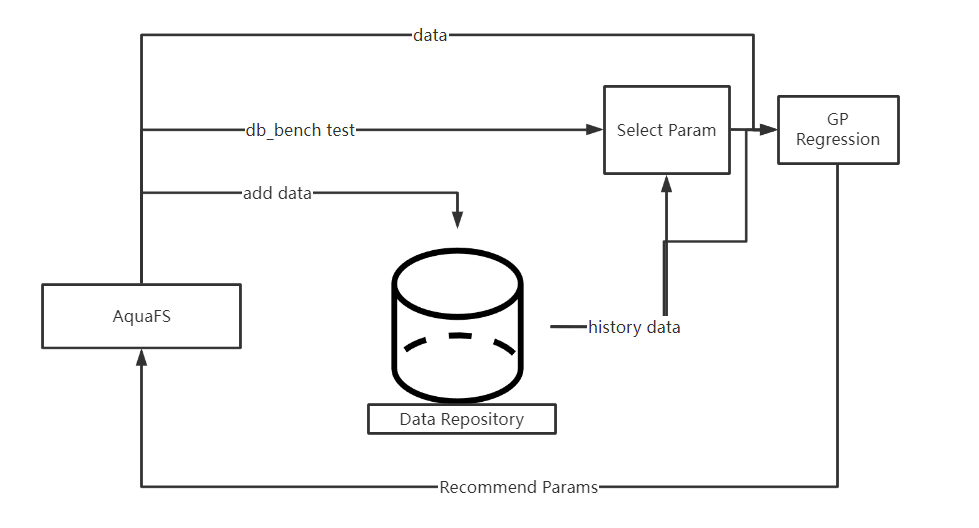
\includegraphics[width=0.7\textwidth]{fig/aquaturnner.png}
  \caption{AquaTurnner 智能调参模块}
  \label{aquaturnner}
\end{figure}

如图 \ref{aquaturnner} 所示,AquaTurnner 智能调参模块主要由三部分组成,被调对象,本文中是AquaFS,历史数据存储仓库,以及调参事务组成,调参事务又包括选择参数选择模块和高斯过程回归调整参数模块。

首先,AquaFS需要预热地运行,收集到不同参数配置下的目标指标,本文中使用的是吞吐量指标,将对应的参数配置和目标指标值存入数据仓库中。在初次预热之后,后续不须要预热,除非加入了新的参数指标。

考虑到AquaFS作为RocksDB的插件存在,在本文中使用RocksDB的测试脚本db\_bench来测试系统的吞吐量,采用prometheus作为收集数据的工具。在这个测试中,用收集到的目标指标值和配置参数值,配合历史数据仓库中的数据,来进行参数选择和高斯过程回归。参数选择模块根据方差指标选择最重要的几个参数,高斯过程回归用重要的参数和目标指标值进行拟合以及回归。

首先对于最重要的参数,由方差计算的最大值对应的参数得到:

\begin{equation}
  \label{eq:var}
  \begin{aligned}
    Var(S)=\frac{1}{\lvert S\rvert}\sum_{i=1}^{\lvert S\rvert}(y_i-\mu)^2 \\
    PI(P)=Var(S)-\sum_{i=1}^{N}\frac{S_{P=P_i}}{S}Var(S_{p=p_i})
  \end{aligned}
\end{equation}

这里的 $y_i$ 是样本中的目标值,$\mu$ 是样本目标值均值,$PI$ 系数是基于方差来计算的,即固定某一个参数的值,根据参数的值划分集合,在每个集合中求出集合中目标值的对应方差,再用初始方差 $Var(S)$ 减去这个和,这个 $PI$ 系数越大说明原来的这个参数的影响越大,因为在同一个值的情况下,集合内方差的和很小。

其次由 $CPI$ 指标来选择剩余重要参数:

\begin{equation}
  \label{eq:cpi}
  \begin{aligned}
    CPI(Q|P=p) = Var(S_{P=p})-\sum_{j=1}^{m}\frac{S_{Q=Q_{w_j},P=p}}{S_{P=p}}Var(S_{Q=q_i|P=p})\\
    CPI(Q|P=p) = \max_{1\le i\le n}CPI(Q|P=p_i)
  \end{aligned}
\end{equation}

基于方差的重要参数选择算法如算法 \ref{alg:aquaturnner_select} 所示。

\begin{algorithm}[htb]
  \caption{ AquaTuner参数选择算法 }
  \label{alg:aquaturnner_select}
  \begin{algorithmic}[1]
    \Require
      adjust\_param\_num, db\_bench\_data, data in repository
    \Ensure
      important\_params
    \State important\_params = []
    \State Select the most important param by $PI(param)$, add to important\_params;
    \State For $i$ in adjust\_param\_num $–$ $1$:
    \State \qquad Compute $CPI$ for each param that not in important\_params;
    \State \qquad Select the largest $CPI$’s corresonding params to important params; \\
    \Return important\_params
  \end{algorithmic}
\end{algorithm}

对于连续参数,AquaTuner对于参数指标在参数范围内给出合适的推荐参数值,该合适参数值是在拟合的高斯过程模型曲线上,根据在最优配置参数附近做抖动获得,也即尝试最优配置参数点附近的参数值看目标指标是否有所提升,对于离散参数,AquaTunar尝试匹配最优目标指标值对应的配置参数的离散值。

AquaTuner的运行算法流程如算法 \ref{alg:aquaturnner_trunning} 所示。

\begin{algorithm}[htb]
  \caption{ AquaTuner参数调优算法 }
  \label{alg:aquaturnner_trunning}
  \begin{algorithmic}[2]
    \Require
      adjust\_param\_num
    \Ensure
      recommend\_param
    \State data repository <- warm up system and collect data;
    \State start db\_bench;
    \State db\_bench\_data = collect data from db\_bench;
    \State add db\_bench\_data to data repository;
    \State important\_params = Select\_Param(adjust\_param\_num ,db\_bench\_data, data in repository);
    \State GP\_model = GP\_regression(important\_params, eb\_bench\_data, data in repository);
    \State recommend\_param = [];
    \State For param in  history\_best\_params and important params:
    \State \qquad If param is continuous:
    \State \qquad \qquad Try values near the past value, add to recommend\_param;
    \State \qquad Else if param is discrete:
    \State \qquad \qquad Try values in best params,add to recommend\_param;
    \State Target = GP\_model.predict(recommend\_param);
    \State If Target is better:
    \State \qquad \Return recommend\_param;
    \State \Return history\_best\_param;
  \end{algorithmic}
\end{algorithm}
